\chapter{Garbage collected Programming Languages}

In this chapter, the used garbage collection implementations of two programming
languages are presented. These are implementations of the theoretical concepts
presented in \autoref{sec:overview}

\section{Go}
\section{Java}

Java by default uses a generational garbage collector as introduced in \autoref{sec:gc_generational}.
This garbage collector is called Garbage First (G1) and was made the default with Java 9 \cite{java_gc_comparison_2018}.
Before that, Java used various types of mark and sweep collectors \cite{java_available_gcs}.

Beyond those there are many more garbage collectors available for Java that can
be used by specifying them as a command line argument to the JVM.
These are not relevant for this writing, as they are not used by default.
Nonetheless these can be very useful when wanting to use a garbage collector
tuned to a specific use case.

\subsection{Garbage First Collector introduction}

Contrary to the theoretical concept of a generational garbage collector,
the memory areas for each generation in G1GC are not continuous in memory.
Instead G1GC uses a heap divided into regions usually 1 MB - 32 MB in size.
Each region is assigned to one of the generations or unused.
These generations are called Eden, Survivor and Old. \cite{java_g1_getting_started}
An example heap layout with regions assigned to the generations is shown in \autoref{fig:g1_heap_layout}.

\begin{figure}[htbp]
    \centering
    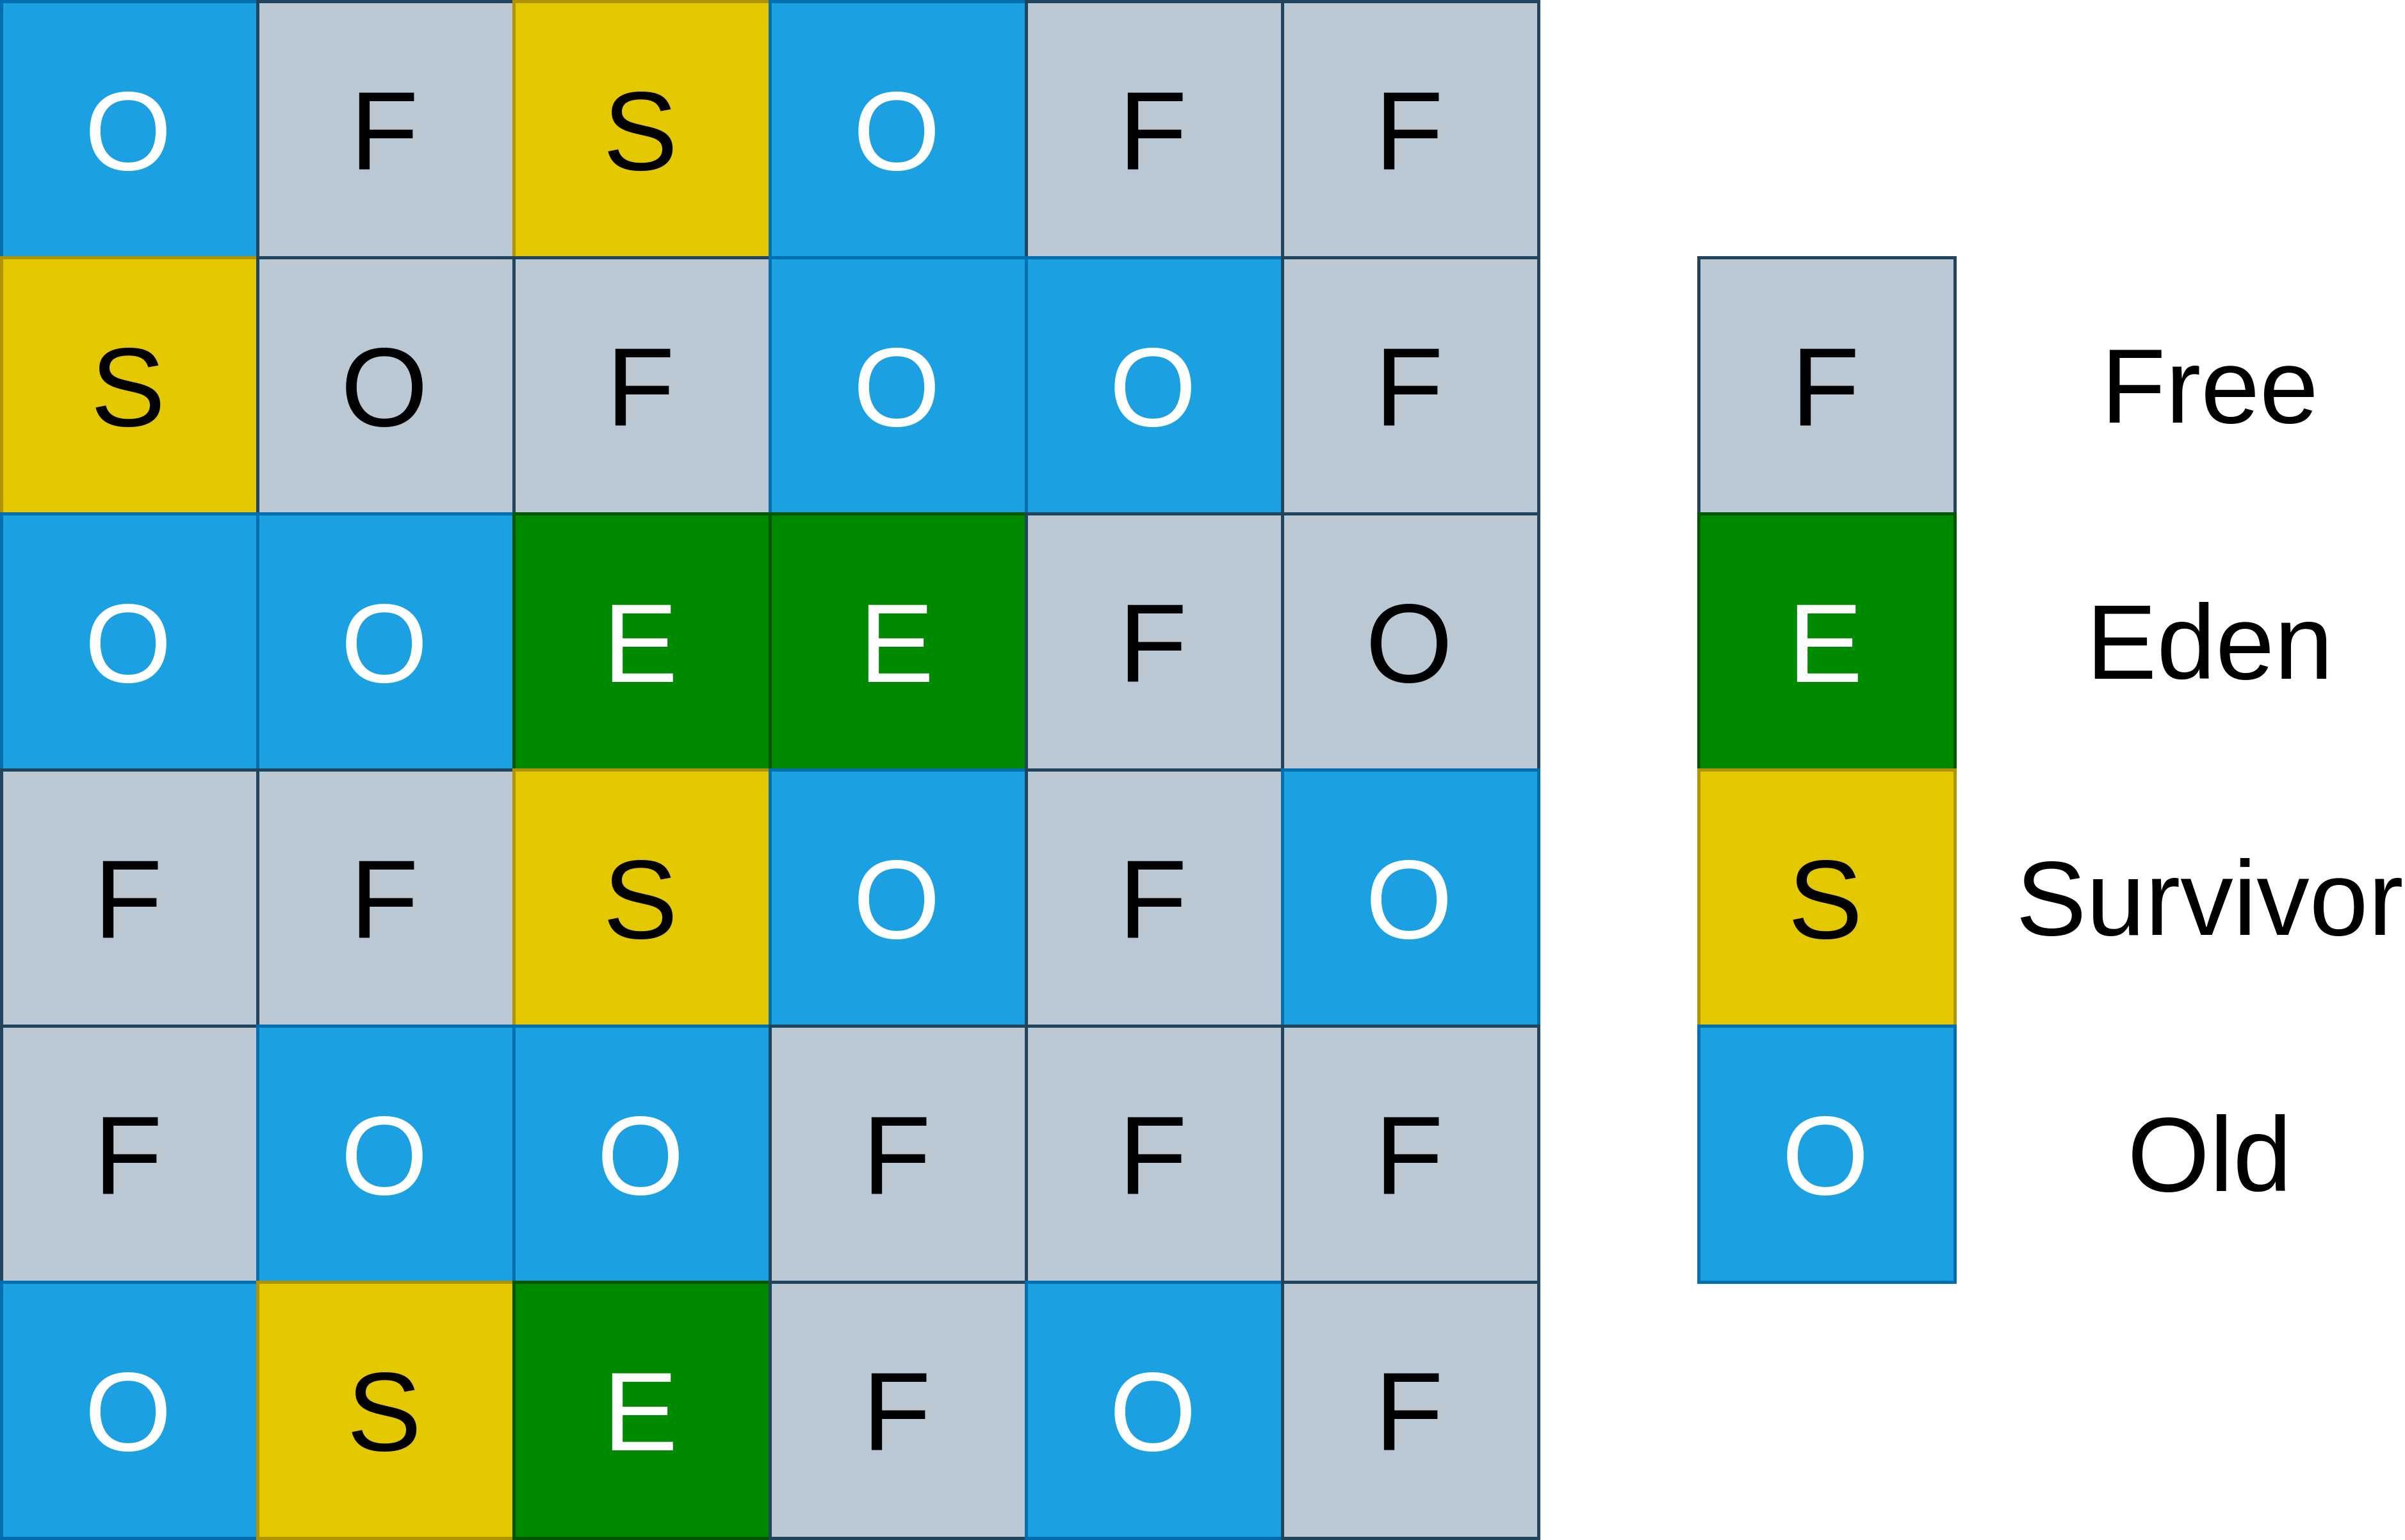
\includegraphics[width=.7\textwidth]{images/G1_Heap_Layout.drawio.png}
    \caption{Heap layout of the G1 garbage collector}
    \label{fig:g1_heap_layout}
\end{figure}

Using constant sized regions instead of continuous memory areas has the advantage
that the heap does not need to be contiguous in memory for generational garbage collection to work.

\subsection{Allocating memory}

When a object is allocated onto the heap, it will be first allocated into the
Eden region inside of the Young generation as outlined in the theoretical concept
of generational garbage collection in \autoref{sec:gc_generational}.
One memory region is marked as the current allocation region.
New objects are allocated into this region until.
Once the region is full, it will be marked as full and a new currently unused region will be
chosen as the new allocation region \cite[2.1 Allocation]{java_g1_2004}.
If no free memory region is available, a new one will be allocated through the operating system.

Large objects are stored in their own regions, called humongous regions
and not inside the Young/Old generation regions.
This is done to simplify the garbage collection of large objects which
would cause problems when stored inside the Young/Old generation regions \cite[2.1 Heap Layout]{java_g1_2004}.

\subsection{Collecting memory from memory regions}

% TODO: compacting

\subsection{Realtime goal of G1}

G1 tries have low pause times for garbage collection improving the
responsiveness of the application and allow for usage in applications
requiring predictable pause times. However pause times are only goals
and there are no guarantees that they will be met
\cite[3.2 Satisfying a Soft Real-Time Goal]{java_g1_2004}.

It does this by estimating the amount of garbage in each region and
prioritizing regions with more garbage for collection, resulting in lower stop-the-world mark phases
compared to regions with less garbage. % TODO: source
Additionally it predicts how long a collection of a region will take and
limit the amount that is done in a garbage collection cycle to meet a
specified time goal \cite[3.2.1 Predicting Evacuation Pause Times]{java_g1_2004}.

The pause time goal and desired intervals for garbgage collection pauses can be configured using
JVM command line arguments \cite[Ergonomic Defaults for G1 GC]{java_g1_getting_started}.

% TODO: shenandoah mention?
